% a-project.tex, v-1.0.3 marcoreis baseado no
% abntex2-modelo-trabalho-academico.tex, v-1.9.7 laurocesar
% Copyright 2012-2018 by abnTeX2 group at http://www.abntex.net.br/ 
% 
% This work consists of the files ........
% 
% -----------------------------------------------------------------------------
% Modelo para desenvolvimento de documentação de projetos acadêmicos
% (tese de doutorado, dissertação de mestrado e trabalhos de monografias em geral) 
% em conformidade com ABNT NBR 14724:2011: Informação e documentação. 
% -----------------------------------------------------------------------------
% Opções para a documentação
%
% Fancy page headings 
%\documentclass[fancyheadings, subook]{Classes/a-prj}
%\documentclass[fancyheadings, sureport]{Classes/a-prj}
%
% Fancy chapters and sections headings 
%\documentclass[fancychapter, subook]{Classes/a-prj}
%\documentclass[fancychapter, sureport]{Classes/a-prj}
%
% Fancy page , chapters and sections headings
%\documentclass[fancyheadings, fancychapter, subook]{Classes/a-prj}
\documentclass[fancyheadings, fancychapter, sureport]{Classes/a-prj}
%
% -----------------------------------------------------------------------------
% Alguns comandos para a fancy page headings)
%
% Page header line width
%\footlinewidth{value}
%
% Page footer line width
%\headlinewidth{value}
%
% Page header and footer line width
%\headingslinewidth{value}
%
% Page header and footer lines without text
%\headingslinesonly
%
% The default line width is 0.3pt.
% Set the value to 0pt to remove the page header and/or footer line
%
% -------------------------------------------------------------------------------
% Formato de figuras suportado
% -------------------------------------------------------------------------------
% O formato das figuras depende da forma como o arquivo de saída é gerado.
% As figuras inseridas na pasta Figures serão automaticamente reconhecidas sem
% a necessidade de inserir a extensão do arquivo.
%
% O pdfLaTEX (PDF) suporta figuras com as extensões: pdf, jpg, png e mps.
%
% -------------------------------------------------------------------------------
% Árvore do diretório a-project.tex
%  Diretório
%       \Classes        (requerido)
%       \Figures        (requerido) --------------------------------->
%       \Figures\PDF    (optional)
%       \Figures\JPG    (optional) Figures located within these
%       \Figures\PNG    (optional) folders are searched automatically
%       \Figures\MPS    (optional)  by the a-prj class.
%       \Figures\EPS    (optional)
%       \Figures\PS     (optional) <--------------------------------
%       \Tables         (requerido)
%       \Others         (requerido)
%       \Chapters       (requerido)
%       \Appendices     (optional)
%       \References     (requerido)
%
% -------------------------------------------------------------------------------
% PDF File resumo
\ifpdf
    \hypersetup{
    	backref,
        colorlinks  = true,
        pdftitle    = Modelo de documentação,
        pdfauthor   = {Marco Reis, marco.a.reis@gmail.com},
        pdfsubject  = Mestre em Engenharia,
        pdfcreator  = Subtitulo,
        pdfproducer = PDFLatex,
        pdfkeywords = {documentação, latex, dissertação, tese}}
 \fi
%
% -------------------------------------------------------------------------------
% Relação de pacotes opcionais utilizados
\usepackage[utf8]{inputenc}
\usepackage[brazil]{babel}
\usepackage{longtable}
\usepackage{dcolumn}
\usepackage{multirow}
\usepackage{lscape}
%\usepackage{graphicx}
\usepackage{rotating}
%\usepackage{float,subfigure}
%\usepackage{graphicx, subfigure}
\usepackage{cite}
\usepackage[left=3cm,top=3cm,right=2cm,bottom=2cm]{geometry}
\usepackage[alf]{abntex2cite}
\usepackage{ifpdf}
\usepackage{shadow}
\usepackage{wrapfig}
\usepackage[normalem]{ulem}
\usepackage{makeidx}
\usepackage{yfonts}
\usepackage{algorithm}
\usepackage{algorithmic}
\usepackage{lmodern}
\usepackage[T1]{fontenc}
\usepackage{indentfirst}
\usepackage{color}
\usepackage{microtype}
\usepackage{lipsum}
\usepackage{caption}
\usepackage{subcaption}
%
\makeindex 
\setlength{\LTcapwidth}{\textwidth}
%
\newtheorem{theorem}{Teorema}
\newtheorem{definition}[theorem]{Definição}
%
% -------------------------------------------------------------------------------
% Configurações do pacote backref
\renewcommand{\backrefpagesname}{Citado na(s) página(s):~}
% Texto padrão antes do número das páginas
\renewcommand{\backref}{}
% Define os textos da citação
\renewcommand*{\backrefalt}[4]{
	\ifcase #1 %
		Nenhuma citação no texto.%
	\or
		Citado na página #2.%
	\else
		Citado #1 vezes nas páginas #2.%
	\fi
}
% 
% -------------------------------------------------------------------------------
% Início do documento raiz
\begin{document}
% Definição do título da página
    \university{Centro Universitário SENAI CIMATEC}
	%\faculty{Programa de...}
	%\school{Escola de...}
% 
    %\course{Engenharia Elétrica}
    \typework{Fundamentos de Robótica Móvel}
% 
	%\course{Mestrado em Modelagem Computacional e Tecnologia Industrial}
	%\typework{Disserta\c{c}\~ao de mestrado}
	%\typework{Exame de Qualificação de Mestrado}
% 
	%\course{Engenharia Elétrica}
	%\typework{Tese de doutorado}
	%\typework{Exame de Qualificação de doutorado}
%
% -------------------------------------------------------------------------------
% Informações gerais
    \thesistitle{Desenvolvimento do robô móvel.}
    \hidevolume
    \thesisvolume{Volume 1 of 1}
    \thesisauthor{Michael Faraday}
    \thesisauthorr{John Nash}
    \thesisauthorrr{James Clerk Maxwell}
    \thesisauthorrrr{Nikola Tesla}
    \thesisauthorrrrr{Sir Isaac Newton}
    %\thesisadvisor{Prof. Marco Reis, M.Eng.}
    %\hidecoadvisor
    %\thesiscoadvisor{Marco Reis}
    \thesisdegreetitle{Bacharel em Engenharia}
    \thesismonthyear{Agosto de 2020}
% 
    \maketitlepage
%
% ----------------------------------------------------------------------------
% Inserir Folha de rosto, Nota de estilo, folha de assinaturas, dedicatoria
    \begin{folharosto}

\begin{center}
\theauthor \\
\theauthorr \\
\theauthorrr \\
\theauthorrrr \\
\theauthorrrrr \\
\end{center}
\ \\
\ \\
\ \\
\ \\
\ \\
\begin{spacing}{2}
   \begin{center}
   {\LARGE {\bf \thetitle}}
   \end{center}
\end{spacing}
\ \\
\ \\
\ \\
\vspace*{85mm}
% \begin{flushright}

%    \begin{list}{}{
%       \setlength{\leftmargin}{7.5cm}
%       \setlength{\rightmargin}{0cm}
%       \setlength{\labelwidth}{0pt}
%       \setlength{\labelsep}{\leftmargin}}

%       \item \thetypework apresentada ao \thefaculty, Curso de \thecourse
%       do \theuniversity, como requisito parcial para a obten\c{c}\~ao do
%       t\'itulo de {\bf \thedegreetitle}.

%       \begin{list}{}{
%       \setlength{\leftmargin}{0cm}
%       \setlength{\rightmargin}{0cm}
%       \setlength{\labelwidth}{0pt}
%       \setlength{\labelsep}{\leftmargin}}

%       \item \'Area de conhecimento: Interdisciplinar

%       \item Orientador: \theadvisor
%       \newline \hspace*{2.1cm}  %{\it \theuniversity}

%       \end{list}
%    \end{list}

% \end{flushright}
\ \\
\ \\
\ \\
\ \\
%\begin{spacing}{1.5}
   \begin{center}
   Salvador \par
   \theuniversity \par
   2020
   \end{center}
%\end{spacing}

\end{folharosto}

    %\begin{notaestilo}
Esta \thetypeworkthree foi elaborada considerando as normas de
estilo (i.e. est\'eticas e estruturais) propostas aprovadas pelo
colegiado do \thefacultytwo e est\~ao dispon\'iveis em formato
eletr\^onico ({\it download} na P\'agina Web
http:$//$ead.fieb.org.br$/$portal\_faculdades$/$dissertacoes-e-teses-mcti.html
ou solicita\c{c}\~ao via e-mail \`a secretaria do
programa) e em formato impresso somente para consulta. \\

Ressalta-se que o formato proposto considera diversos itens das
normas da Associa\c{c}\~ao Brasileira de Normas T\'ecnicas (ABNT),
entretanto opta-se, em alguns aspectos, seguir um estilo pr\'oprio
elaborado e amadurecido pelos professores do programa de
p\'os-gradua\c{c}\~ao supracitado.

\end{notaestilo}

    %\begin{folhaassinaturas}

%\thispagestyle{empty}

\def\signature#1#2{\parbox[b]{1in}{\smash{#1}\vskip12pt}
\hfill \parbox[t]{3in}{\shortstack{\vrule width 3in height
0.4pt\\\small#2}}}

\def\InstituicaoMembro#1#2{\parbox[b]{1in}{\smash{#1}\vskip12pt}
\hfill \parbox[t]{3in}{\shortstack{\vrule width 3in \\\small#2}}}

\def\signaturepage{%

    \begin{spacing}{1.5}
        \begin{center}
        {\LARGE \theuniversity} \\
        {\large \thefaculty} \\
        {\large \thecourse} \\
        \end{center}
    \end{spacing}

   \vskip 0.25in plus 0.4in minus 0.1in

    \begin{spacing}{1.5}
        \begin{sloppypar}
        A Banca Examinadora, constitu\'ida pelos professores abaixo
        listados, leram e recomendam a aprova\c{c}\~ao [com distin\c{c}\~ao] da
        \thetypeworktwo, intitulada ``\thetitle",
        apresentada no dia (dia) de (m\^es) de (ano), como requisito
        parcial para a obten\c{c}\~ao do t\'itulo de {\bf \thedegreetitle}.\\
        \end{sloppypar}
    \end{spacing}

    \def\sigskip{\vskip0.15in plus 0.2in minus 0.1in}
    \def\beginskip{\vskip0.3875in plus 0.2in minus 0.1in}

    \beginskip
    \signature{Orientador:}{Prof. Dr. \theadvisor} \\
    \InstituicaoMembro{}{\theuniversity} \\

    \sigskip
    \beginskip
    \signature{Membro externo da Banca:}{Prof. Dr. Nome completo} \\
    \InstituicaoMembro{}{Institui\c{c}\~ao do membro da banca} \\

    \sigskip
    \beginskip
    \signature{Membro externo da Banca:}{Prof. Dr. Nome completo} \\
    \InstituicaoMembro{}{Institui\c{c}\~ao do membro da banca} \\

    %\sigskip
    %\beginskip
   % \signature{Membro interno da Banca:}{Prof. Dr. Nome completo} \\
   % \InstituicaoMembro{}{Institui��o do membro da banca} \\

    \vfill
    \newpage
    \setcounter{page}{3}
}
%*********************************************************************


\signaturepage


\end{folhaassinaturas}

    %\include{Others/dedicatoria}
    %\include{Others/agradecimentos}
%
% ----------------------------------------------------------------------------
% Resumo/abstract, sumário e siglas
    \begin{romanpagenumbers}
        \begin{thesisresumo}
Escreva aqui o resumo da disserta\c{c}\~ao, incluindo os contextos geral e espec\'ifico, dentro dos quais a pesquisa foi realizada, o objetivo da pesquisa, assun\c{c}\~ao filos\'ofica, os m\'etodos de pesquisa usados e as poss\'iveis contribui\c{c}\~oes que o que \'e proposto pode trazer \`a sociedade.

\ \\

% use de três a cinco palavras-chave

\textbf{Palavras-chave}: Palavra-chave 1, Palavra-chave 2, Palavra-chave 3, Palavra-chave 4, Palavra-chave 5

\end{thesisresumo}

        \begin{thesisabastract}
Escreva aqui, em ingl\^es, o resumo da disserta\c{c}\~ao, incluindo os contextos geral e espec\'ifico, dentro dos quais a pesquisa foi realizada, o objetivo da pesquisa, assun\c{c}\~ao filos\'ofica, os m\'etodos de pesquisa usados e as poss\'iveis contribui\c{c}\~oes que o que \'e proposto pode trazer \`a sociedade. 

\ \\

% use de tr�s a cinco palavras-chave

\textbf{Keywords}: Keyword 1, Keyword 2, Keyword 3, Keyword 4, Keyword 5

\end{thesisabastract}

        % Make list of contents, tables and figures
        \thesiscontents
        %Include other required section
        %\begin{thesisabbreviations}
\begin{footnotesize}
\begin{longtable}[l]{p{2cm}l}
  tprax   \dotfill & \thefaculty \\
  WWW       \dotfill &  World Wide Web \\
\end{longtable}
\end{footnotesize}
\end{thesisabbreviations}

        %\begin{thesissymbols}
\begin{footnotesize}
\begin{longtable}[l]{p{2cm}l}
  $\partial$   \dotfill  & Bla bla bla \\
  $\prod$       \dotfill & ble ble ble \\
  $\partial$   \dotfill  & Bla bla bla \\
  $\prod$       \dotfill & ble ble ble \\
  $\partial$   \dotfill  & Bla bla bla \\
  $\prod$       \dotfill & ble ble ble \\
  $\partial$   \dotfill  & Bla bla bla \\
  $\prod$       \dotfill & ble ble ble \\
  $\partial$   \dotfill  & Bla bla bla \\
  $\prod$       \dotfill & ble ble ble \\
  $\partial$   \dotfill  & Bla bla bla \\
  $\prod$       \dotfill & ble ble ble \\
  $\partial$   \dotfill  & Bla bla bla \\
  $\prod$       \dotfill & ble ble ble \\
  $\partial$   \dotfill  & Bla bla bla \\
  $\prod$       \dotfill & ble ble ble \\
  $\partial$   \dotfill  & Bla bla bla \\
  $\prod$       \dotfill & ble ble ble \\
  $\partial$   \dotfill  & Bla bla bla \\
  $\prod$       \dotfill & ble ble ble \\
  $\partial$   \dotfill  & Bla bla bla \\
  $\prod$       \dotfill & ble ble ble \\
  $\partial$   \dotfill  & Bla bla bla \\
  $\prod$       \dotfill & ble ble ble \\
  $\partial$   \dotfill  & Bla bla bla \\
  $\prod$       \dotfill & ble ble ble \\
  $\partial$   \dotfill  & Bla bla bla \\
  $\prod$       \dotfill & ble ble ble \\
  $\partial$   \dotfill  & Bla bla bla \\
  $\prod$       \dotfill & ble ble ble \\
  $\partial$   \dotfill  & Bla bla bla \\
  $\prod$       \dotfill & ble ble ble \\
  $\partial$   \dotfill  & Bla bla bla \\
  $\prod$       \dotfill & ble ble ble \\
  $\partial$   \dotfill  & Bla bla bla \\
  $\prod$       \dotfill & ble ble ble \\
  $\partial$   \dotfill  & Bla bla bla \\
  $\prod$       \dotfill & ble ble ble \\          
\end{longtable}
\end{footnotesize}
\end{thesissymbols}

        %Switch the page numbering back to the default format
    \end{romanpagenumbers}
%
% ---------------------------------------------------------------------------
% Include thesis chapters
    \parskip=\baselineskip
    \chapter{Introdução}
\label{chap:intro}

A odometria \'e uma t\'ecnica usada para medir a dist\^ancia percorrida. Sendo de grande import\^ancia no ramo da Rob\'otica, pois \'e imprescind\'ivel que um rob\^o m\'ovel consiga se locomover de maneira a alcan\c{c}ar o seu ponto de destino.
Para tal, \'e necess\'ario que este rob\^o possua uma forma de se localizar no espa\c{c}o, atrav\'es de algum sensor que lhe d\^e esta informa\c{c}\~ao.
\'E importante tmb\'em que ele possa evitar situa\c{c}\~oes perigosas, como colis\~oes, buracos e locais com condi\c{c}\~oes clim\'aticas prejudicias ao rob\^o. De forma, a alcan\c{c}ar o local desejado.
Al\'em disso, ele deve registrar ou j\'a ter registrado o mapa do local em que se encontra e ser capaz de interpretar esta informa\c{c}\~ao para ser utilizada ao seu favor, fazendo com que o mesmo consiga se deslocar no ambiente de forma segura at\'e encontrar a sua meta.

%--------- NEW SECTION ----------------------
\section{Objetivos}
\label{sec:obj}

Estudar o funcionamento da tecnologia Pozyx para aferi\c{c}\~ao do posicionamento de um rob\^o m\'ovel, de forma a auxiliar a odometria do mesmo.


\subsection{Objetivos Específicos}
\label{ssec:objesp}

Estudar funcionamento do Pozyx;
Descrever a forma de utiliza\c{c}\~ao do posicionamento para odometria do ro\^o;
Pesquisar as suas diferen\c{c}as para outras tecnologias de aux\'ilio a odometria;
Buscar as aplica\c{c}\~oes do Pozyx na rob\'otica.


%--------- NEW SECTION ----------------------
\section{Justificativa}
\label{sec:justi}

O Pozyx \'e uma solu\c{c} de hardware e software que fornece informa\c{c}\~oes precisas de posicionamento e movimento com boa precis\~ao.
Esta precis\~ao s\'o p\^ode ser alcan\c{c}ada devido a sua tecnologia de banda ultralarga, algoritmos inteligentes e aprendizado da m\'aquina.
Logo, o estudo da utiliza\c{c}\~ao do Pozyx \'e imprescind\'ivel para t\^e-lo como op\c{c}\~ao na aferi\c{c}\~ao do posicionamento do ro\^o para a odometria adequada do mesmo. 


%--------- NEW SECTION ----------------------
\section{Organização do documento}
\label{section:organizacao}

Este documento apresenta $5$ capítulos e está estruturado da seguinte forma:

\begin{itemize}

  \item \textbf{Capítulo \ref{chap:intro} - Introdução}: Contextualiza o âmbito, no qual a pesquisa proposta está inserida. Apresenta, portanto, a definição do problema, objetivos e justificativas da pesquisa e como este \thetypeworkthree está estruturado;
  \item \textbf{Capítulo \ref{chap:fundteor} - Fundamentação Teórica}: Descreve o funcionamento do Pozyx e aborda as diferenças das outras tecnologias;
  \item \textbf{Capítulo \ref{chap:mat} - Materiais e Métodos}: ;
  \item \textbf{Capítulo \ref{chap:result} - Resultados}: ;
  \item \textbf{Capítulo \ref{chap:conc} - Conclusão}: Apresenta as conclusóes, contribuições e algumas sugestões de atividades de pesquisa a serem desenvolvidas no futuro.

\end{itemize}

    \chapter{Fundamentação Teórica}
\label{chap:fundteor}

\begin{flushright}

   \begin{list}{}{
      \setlength{\leftmargin}{4.5cm}
      \setlength{\rightmargin}{0cm}
      \setlength{\labelwidth}{0pt}
      \setlength{\labelsep}{\leftmargin}}
      \item Quanto maior for a rapidez de transformação de uma
      sociedade, mais temporárias são as necessidades
      individuais. Essas flutuaçõess tornam ainda mais acelerado
      o senso de turbilh da sociedade.

      \begin{list}{}{
      \setlength{\leftmargin}{0cm}
      \setlength{\rightmargin}{0cm}
      \setlength{\labelwidth}{0pt}
      \setlength{\labelsep}{\leftmargin}}
      \item (Alvin Toffler)
      \end{list}
   \end{list}
\end{flushright}

\begin{flushright}
  Quanto maior for a rapidez de transformação de uma \\
  sociedade, mais temporárias são as necessidades \\
  individuais. Essas flutuações tornam ainda mais \\
  acelerado o senso de turbilhão da sociedade. \\
  \ \\
  (Alvin Toffler)
\end{flushright}

%--------- NEW SECTION ----------------------
\section{Ultra Wide Band}
\label{sec:sota}
O princípio de funcionamento do Pozyx se dá na utilização da tecnologia 
de Ultra Wide Band (UWB) ou de banda ultra larga. UWB é um protocolo de comunicação sem fio
assim como o Wi-fi e o Bluetooth. Contudo, seu funcionamento difere um pouco destas e outras tecnologias,
trazendo vantagens e desvantagens. O uso e os estudos acerca da tecnologia UWB vêm se desenvolvendo
há cerca de 100 anos, quando o inventor e físico italiano Guglielmo Marconi (1874-1937), baseando-se na teoria 
de Maxwell sobre ondas eletromagnéticas, estudava os princípios da transmissão de dados por radiofrequência. Futuramente 
foi utilizada em radares do exército estado-unidense e, entre os anos de 1960 a 1990 ficou restrita aplicações militares.

%--------- NEW SECTION ----------------------
\section{Características da tecnologia}
\label{sec:ass1}
Como mencionado anteriormente, a tecnologia UWB possui algumas diferenças de funcionamento,
quando comparada a outras de comunicação \textit{Wireless}. 

\subsection{Vantagens}
Sua principal vantagem é a larga banda de frequência na qual pode operar: aproximadamente 500 MHz, 
enquanto as do Wi-fi e Bluetooth são de algumas dezenas de MHz. Essa grande largura de banda torna 
os sinais menos susceptíveis a interferências, oriunda de ondas emitidas por outros aparelhos ao redor.
A Figura 2.1 ilustra essa diferença.

\begin{figure} [h!]												 
	\centering													 
	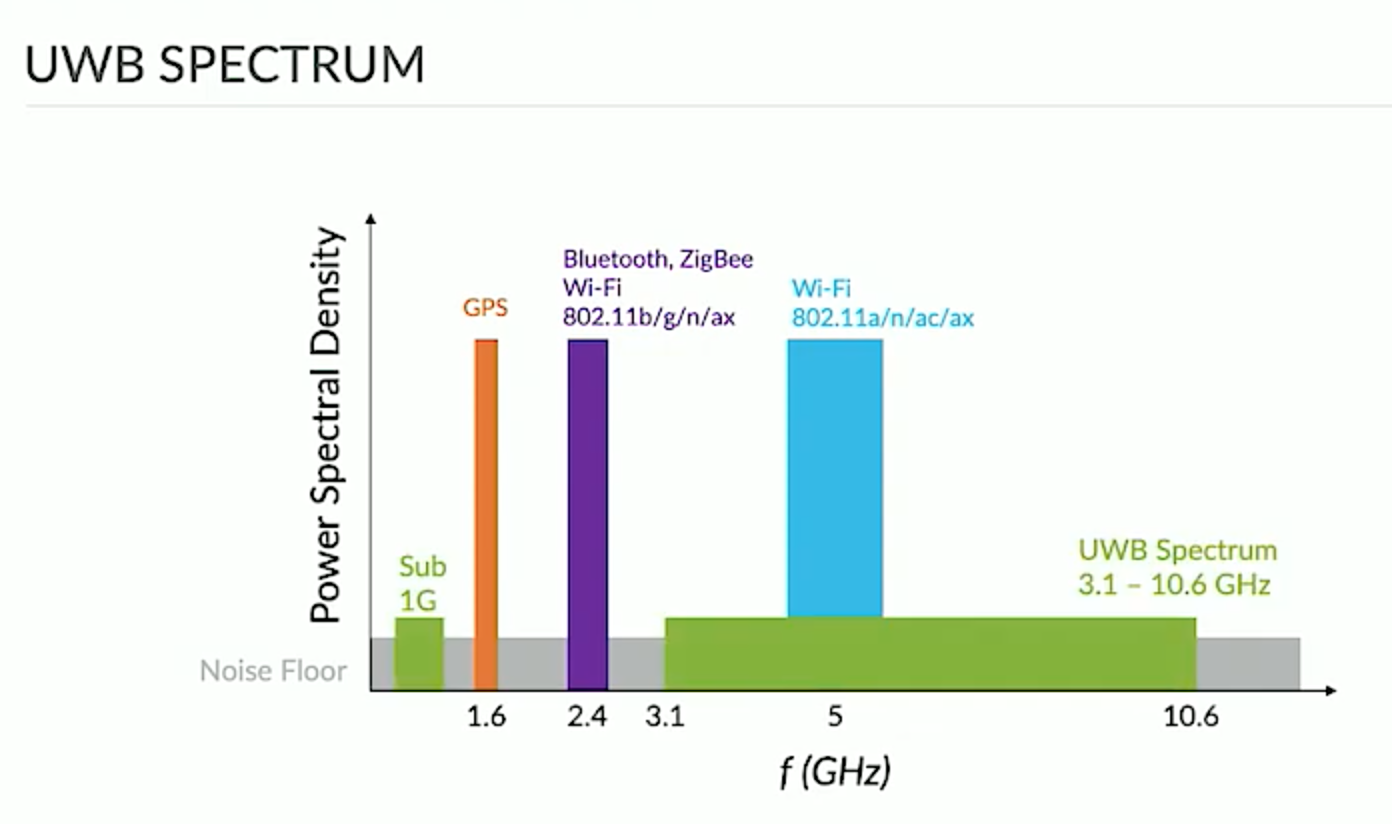
\includegraphics[width=0.8\textwidth]{./uwb_spectrum}				 
	\caption{Insufficient data.}		
	\label{img:ihuma}												 
\end{figure}

Outra característica do UBW é a utilização de rápidos pulsos (em média 2 ns entre as bordas de subida e descida) para transmitir dados, 
que são muito mais eficientes e precisos do que por alteração da frequência ou amplitude do sinal. Essa é uma das características
que fazem desta tecnologia muito útil para localização \textit{indoor}, podendo apresentar uma precisão de menos de 15 cm,
quanto outras tecnologias não chegam a 1 metro.

Uma das grandes dificuldades em localização \textit{indoor} é a perda do sinal ao ser refletido em paredes ou outros obstáculos. Considerando sinais
senoidais, a interferência entre o sinal emitido e refletido pode alterar o sinal a ponto de sua frequência e amplitude não serem
mais reconhecidas pelo receptor. Por utilizar pulsos e trabalhar numa ampla faixa de frequência, os sinais do UWB se mostram mais 
eficientes nessas situações, visto que são menos susceptíveis a estas alterações. 

Como pode ser visto na imagem acima, o UWB trabalha em uma potência significativamente mais baixa do que as outras tecnologias em 
toda sua banda, o que deixa aparelhos alimentados por baterias, como robôs móveis, muito mais eficientes, visto que gastariam menos energia
para se localizar.

\subsection{Desvantagens}
Em contrapartida às características supracitadas, UWB ainda têm sua aplicabilidade restrita por alguns fatores.
Por ser uma tecnologia ainda não muito explorada no mercado, seus equipamentos de instalação ainda são caros. Além disso,
o alcance máximo de um sinal em UWB é de, em média, 10 metros, tornando necessário o posicionamento de vários \textit{anchors} para que
o posicionamento em locais grandes se torne eficiente, o que encarece ainda mais o sistema.

\section{Aplicações na robótica}
A tecnologia Pozyx se assemelha com as RFID e BLE, pois para a localização de um objeto utiliza-se a estratégia de introduzir um elemento que emita um sinal e outro que capta este sinal. Estes elementos são as tags e as âncoras (anchors), o primeiro elemento se encontra no objeto e as âncoras são referências que possuem localização conhecida pelo servidor no ambiente. 

Nesta implementação, uma estratégia sugerida é chamada de variação bidirecional (TWR), na qual a tag envia um conjunto de sinais que irá atingir as âncoras ao redor e retornar,  de modo que a distância é calculada com base no tempo de viagem do sinal (TOF), uma vez que a velocidade de uma onda de rádio é conhecida. Vale ressaltar, que este processo é validado somente quando a tag consegue atingir três ou mais âncoras, pois assim o objeto irá se encontrar entre a melhor interseção dos raios dos elementos de referência, este procedimento é chamado de triangulação. Entretanto, quando há mais tags no ambiente, um elemento é tomado como referência para os demais, master tag, pois irá receber a localização das demais e se conectar a um servidor. Outra estratégia oferecida pelo fabricante é a Diferença de horário de chegada (TDOA), na qual as tags irão apenas irão apenas transmitir periodicamente um pulso UWB, e não mais esperar um retorno. Este sinal incluirá um ID da tag e será captado por todas as âncoras no alcance, as quais irão transmitir ao servidor, por meio de linhas de Ethernet, o momento exato que cada uma identificou a tag, sendo assim, com base na diferença destes horários  é possível estimar a posição da tag por meio da interseção das hipérboles definidas pelas diferenças de tempos. Nesta operação é imprescindível que a assim como a localização das âncoras sejam conhecidas, os relógios entre elas devem estar sincronizados com muita precisão. A TDOA é uma ótima opção ao considerar situações com altas taxas de atualização de informações. 

De modo geral, a tecnologia possui um grau de precisão bom, porém assim como todo método de localização, ainda se possui erros. Desse modo, em estudos recentes foi possível diminuí-los utilizando algoritmos para a diminuição de erro como o EFK, Extended Kalman Filter,\cite{Um} o qual calcula uma aproximação linear para um conjunto de funções não lineares com base na expansão de Taylor de primeira ordem.

Além da localização de robôs em ambientes indoors, o Pozyx tem estado também em aplicações de logísticas nos setores industriais, como em um estudo de caso \cite{Dois} em que uma determinada empresa possuía uma má administração do  armazenamento de produtos diversos e em pequenos lotes. Neste caso, com a implementação de um sistema de identificação de paletes, utilizando tal tecnologia, foi possível mapear o armazém, sendo assim, a operação reduziu a quantidade de erros, graças a precisão da localização das mercadorias, o que ocasionou um aumento de eficiência no armazém em 3%.

Além dessa aplicação, a tecnologia foi também comprovada em uma situação de extrema movimentação, como nos esportes, quando foi utilizada para a localização de jogadores em \cite{Tres}. Neste estudo foram implementados também algoritmos de filtragem, filtro de kalman e filtro de partículas, o qual resultou em um erro de localização de 31\%, com erros médios de 20 cm. 




%---------------picture------------------------------------
% \begin{figure}
%     \centering
%     \subfigure[Figure A]{\label{fig:a}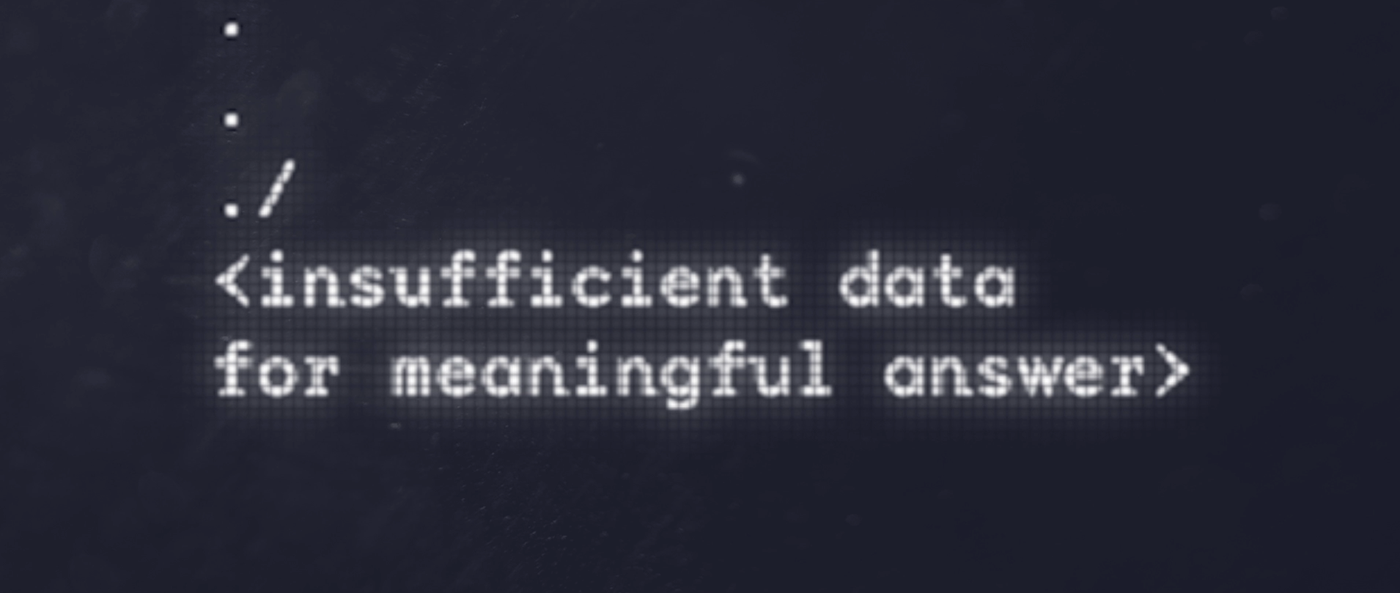
\includegraphics[width=60mm]{./lq}}
%     \subfigure[Figure B]{\label{fig:b}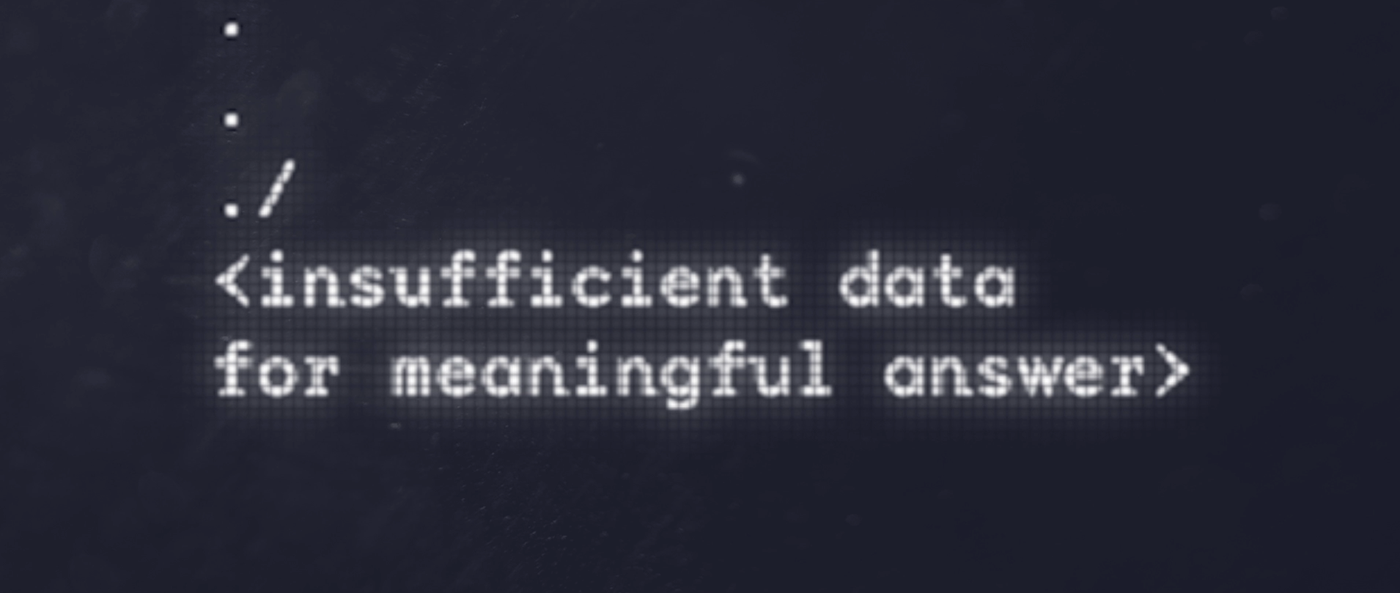
\includegraphics[width=60mm]{./lq}}
%     \subfigure[Figure C]{\label{fig:c}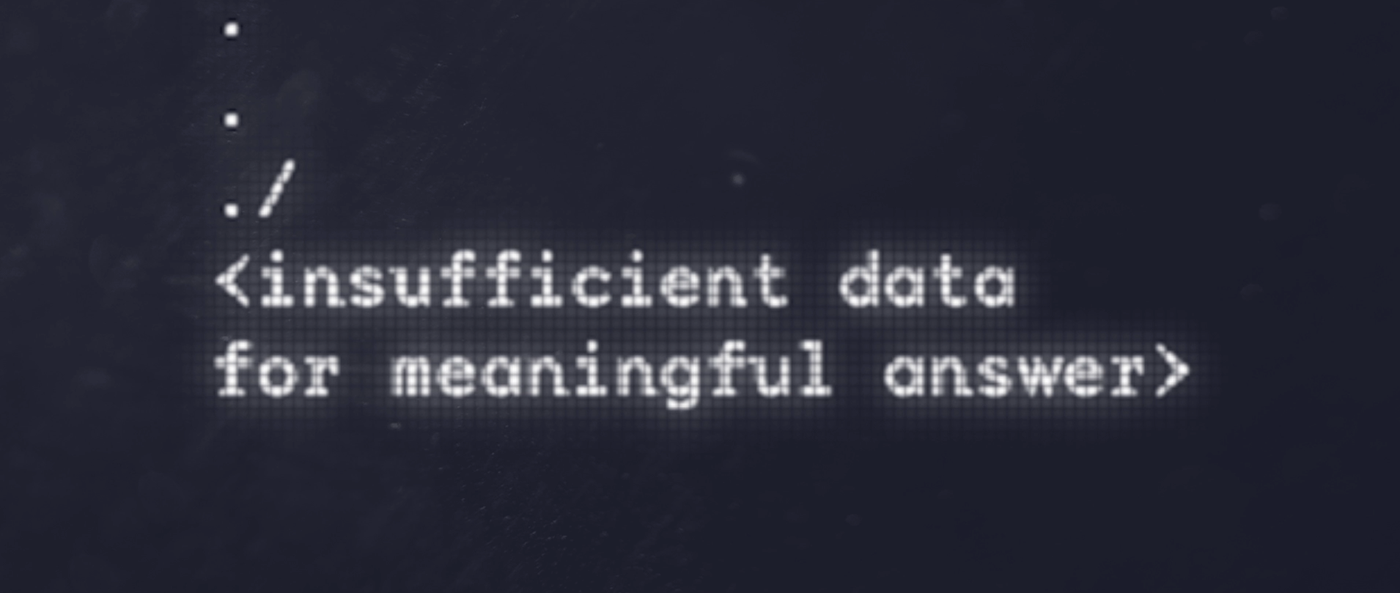
\includegraphics[width=\textwidth]{./lq}}
%     \caption{Three simple graphs}
%     \label{fig:three graphs}
% \end{figure}
%----------------------------------------------------------
    \chapter{Materiais e Métodos}
\label{chap:mat}
\lipsum[1]

\section{Metodologia}
\label{sec:met}
\lipsum[1]

%--------- NEW SECTION ----------------------
\section{Interface do Usuário}
\label{sec:ui}
\lipsum[1]

%--------- NEW SECTION ----------------------
\section{Simulação do sistema}
\label{sec:sim}
\lipsum[2-4]


    \chapter{Resultados}
\label{chap:result}
Importante sempre ter um parágrafo introdutório para explicar os resultados encontrados.

%--------- NEW SECTION ----------------------
\section{Testes unitários}
\label{sec:testu}
\lipsum[1]

\section{Integração do sistema}
\label{sec:intsis}
\lipsum[1]

%--------- NEW SECTION ----------------------
\section{Testes integrados}
\label{sec:testi}
\lipsum[1]








    \chapter{Conclusão}
\label{chap:conc}

O sistema de localização de corpos em ambientes indoor requer uma boa precisão na estimativa de pequenas distâncias, assim como ferramentas capazes de diferenciar freq. Desse modo, conforme apresentado a tecnologia Pozyx ao utilizar a UWB apresenta um bom desenvolvimento, uma vez que é menos susceptíveis a interferências por sinais refletidos e posicionar o robô de forma adequada, além de apresentar uma eficiência energética melhor do que as demais tecnologias apresentadas no mercado. Ademais, possui também como vantagem uma implementação, apesar de robusta, de fácil entendimento e monitoramento e manutenção remotas. Inclusive, apresenta melhor performance quando está relacionada com outras ferramentas de diminuição de erros, como os filtros. Sendo assim, essa ferramenta de localização têm um elevado potencial de desenvolvimento futuro, em diversas aplicações, inclusive em ambientes outdoors, a partir do momento que consiga atingir um alcance maior de transmissão de sinais e, com isso, baratear os custos da aplicação desta tecnologia.

\section{Considerações finais}
\label{sec:consid}




    % include more chapters ...
%
% ----------------------------------------------------------------------------
% Include thesis appendices
    \begin{thesisappendices}
        % Thesis Appendix -------------------------------------------------------

\chapter{Diagramas mecânicos}
\label{Append:diagmec}



        % Thesis Appendix -------------------------------------------------------

\chapter{Diagramas eletro-eletrônicos}
\label{Append:diagele}



        % Thesis Appendix -------------------------------------------------------

\chapter{Logbook}
\label{Append:log}



    \end{thesisappendices}
%
% ----------------------------------------------------------------------------
% Configurar as referencias bibliograficas
	\renewcommand\bibname{Referências}
    \addcontentsline{toc}{chapter}{Referências}
    \bibliography{References/referencias}
%
% ----------------------------------------------------------------------------
% Finishing him
    \include{Others/ultimafolha}
\end{document}
%
% -------------------------------------------------------------------------------
% Aqui termina a formatação para o documento.
% In God We Trust. All Other Bring Data. 
%
% -------------------------------------------------------------------------------